\documentclass[12pt]{article}
\usepackage{hyperref}
%\usepackage{a4wide}
\usepackage[margin=0.8in]{geometry}
\usepackage{graphicx}
\usepackage{wrapfig}
\usepackage{mhchem}
\newcommand{\lambdabar}{{\mkern0.75mu\mathchar '26\mkern -9.75mu\lambda}}
\date{}
\title{\LARGE \bf Nuclear and Particle Physics\\[5mm]Nuclear Physics}
\author{Daniel Ma\^{i}tre, IPPP, Durham University}

\newcommand{\V}[1]{\mathbf{#1}}
\newcommand{\GeV}{\,\rm{GeV}}
\newcommand{\mb}{\, \rm{mb}}
\newcommand{\barn}{\,\rm{b}}
\begin{document}
\maketitle
%
%
%
%
%%\section{Nuclear Masses and Binding Energies}
%%\lecture{1}
\section{Nuclear masses and binding energies}
%
%
%
%
%
%
Atoms are constituted of electron and the atomic nucleus. The nucleus is composed of protons and neutrons (they are referred to as \emph{nucleons}). The protons and neutrons have approximately the same mass. The proton is positively charged and the neutron has a neutral charge.

%%\keypoint{Protons and Neutrons are collectively called Nucleons}

The nucleons in the nuclei are bound together by a force much stronger than the repulsion created by the positive charges of the protons. This force, called strong force has been found to have the following characteristics: 
\begin{itemize}
\item It has a short range of the order of a few $\rm fm$.
\item It is attractive, except for a repulsive core for distances smaller than $\simeq 1\,\rm fm$. 
\end{itemize}  

The nuclei are characterised by
\begin{description} 
\item[Atomic number:] the number of protons in the nucleus. Because the number of proton is the same as the number of electrons in a neutral atom the atomic number specifies the chemical properties of the atom. It is normally denoted with $Z$   
\item[Mass number:] the number of proton and neutrons. As its name suggests it is roughly related to the mass of the nucleus in atomic mass units. It is usually denoted with $A$.
\end{description}

%%\keypoint{Nuclei are characterised by their Atomic and Mass numbers}


A nucleus with atomic number $Z$ and mass number $A$ has therefore $N=A-Z$ neutrons. Nuclides are represented as $\ce{^{A} X}$, $\ce{^{A}_{Z}X}$ or $\ce{^{A}_{Z}X_{N}}$ with $X$ the chemical symbol for the atom. 

The binding energy $B(A,Z)$ of a nucleus with atomic number $Z$ and mass number $Z$ is the difference between its atomic mass and the sum of the mass of its constituents. 
\[M(A,Z)=Z*M(\ce{^{1}H})+(A-Z)M(n)-B(A,Z)\]
(note that by using $m(\ce{^{1}H})$ instead of the proton mass the mass of the electrons are included automatically). This formula assumes that the energy difference coming from the electron binding energies is negligible (it is of the order of a few $\rm{eV}$). 

\begin{figure}
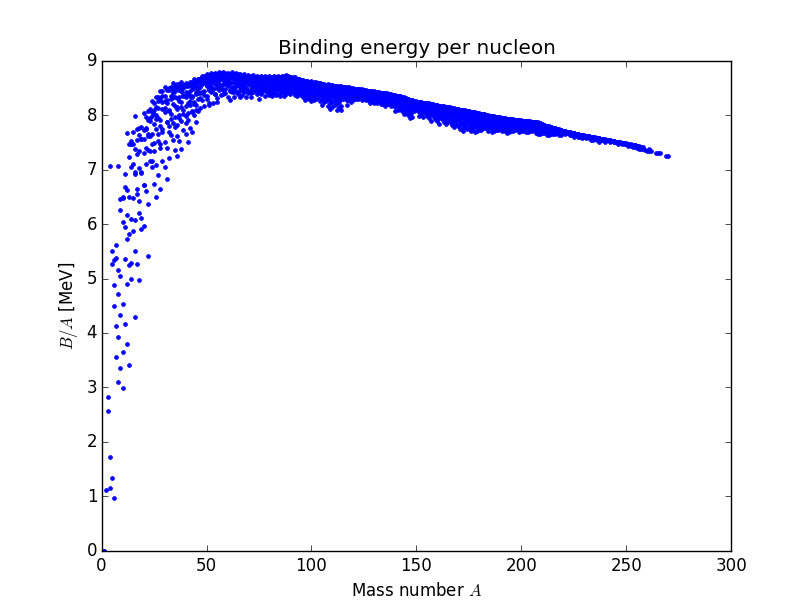
\includegraphics[scale=0.4]{images/BindingEnergyAll.png}
%%\image{BindingEnergyAll.png}
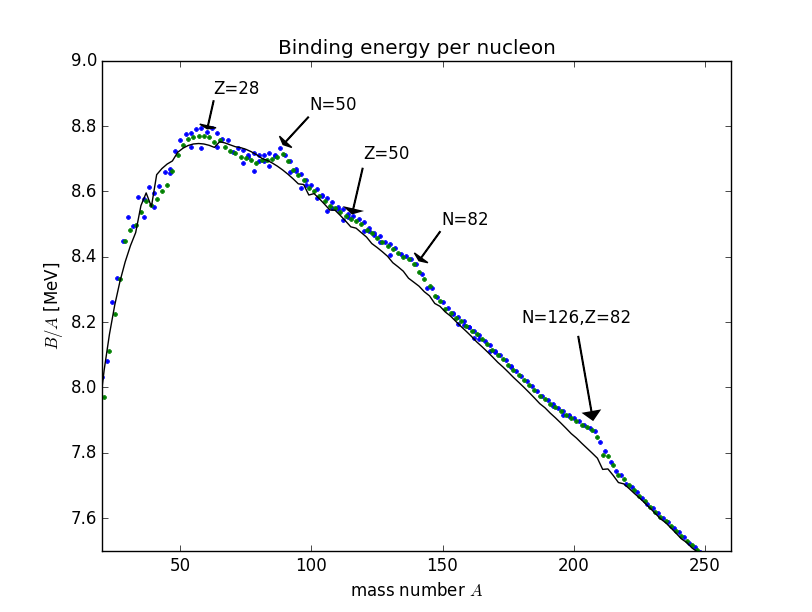
\includegraphics[scale=0.4]{images/BindingEnergyMostStable.png}
\caption{Binding energy per nucleon as a function of the mass number. The first figure shows all nuclides, while the second only shows the most stable isobar. The plain line corresponds to the semi-empirical mass formula eq. \ref{eq:SEMF} for odd $A$ nuclei.}\label{fig:bindingEnergies}
\end{figure}

The binding energies for all nuclei are shown in Fig.~\ref{fig:bindingEnergies}. The binding energies cannot be predicted accurately from first principle but an approximate formula can be postulated based on physical arguments, with parameters to be determined experimentally. 
\begin{equation}\label{eq:SEMF}
M(A,Z)=N M_n+Z M_p+Z\, m_e-a_V A + a_sA^{2/3}+a_c\frac{Z^2}{A^{1/3}}+a_a\frac{(N-Z)^2}{4A}+\frac{\delta}{A^{1/2}}
\end{equation}  

%%\keypoint{The binding energies are calculated with the semi-epirical mass formula}

The first three term are the mass of the constituents of the atom. The remaining term can be justified from a physical argument, but their coefficient has to be determined experimentally. For all terms the nucleus is approximated as sphere whose radius is approximately proportional to $A^{1/3}$.
%%\lecture{2}
\begin{description}
\item[$-a_V A$: ] This is called the volume term. The strong force between nucleons is short-range, unlike the Coulomb force. The consequence is that nucleons only interact with other nucleons that are close enough, so that the contribution to the potential energy is the same for all nucleons and only depend on the density $\rho$ of nucleons in the nucleus. This density is more or less constant for nuclei from moderate to large $A$. The potential energy will be proportional to the number of nucleons and since the density is more or less constant it will be proportional to the volume.  
%%\keypoint{The nuclear force is short range and creates a more or less constant potential within the nucleus volume.} 
\item[$a_sA^{2/3}$:] In the above description we neglected the fact that the density of neighbours is smaller for nucleons at the boundary of the nucleus, these will not contribute as much as those in the middle of the nucleus. This term correct for this effect and is proportional to the area of the nucleus (and hence to $R^2=(A^{1/3})^2=A^{2/3}$).
%%\keypoint{Nucleons at the boundary of the nucleus volume have fewer neighbours and therefore their binding energy is smaller.}
\item[$a_c\frac{Z^2}{A^{1/3}}$:] This is the Coulomb term. The potential for each proton is proportional to the number of other protons so it will be proportional to $Z(Z-1)$. The Coulomb potential is proportional to $1/r$ so we expect a dependence proportional to $1/R=A^{-1/3}$, for large values of $Z$ we can replace $Z(Z-1)$ with $Z^2$.
%%\keypoint{Protons in the nucleus experience a repulsive Coulomb force due to their positive charges.}
\item[$a_a\frac{(N-Z)^2}{4A}$] This is the asymmetry term. Because nucleons have spin $1/2$ they obey Fermi statistics (no two identical nucleon can be in the same state). To illustrate how this term arises we can imagine that the neutrons and protons have the same energy levels, and they fill the lowest $n$ levels if there are $n$ nucleons of one type. If we start from a nucleus with equal number $n$ of protons and neutrons both type will have their $n$ lowest energy state filled. If we now try to replace a neutron with a proton, this cannot work straight-forwardly because the corresponding energy level is already occupied by a proton, so this new proton will have to go into a higher energy level, hence reducing the binding energy. The same happens if we try to exchange a proton with a neutron. A more careful calculation\footnote{see for example \cite{Lilley:2009zz}, p.39 and Appendices B and C} gives the $(Z-N)^2$ dependence but our simplistic argument explains why the asymmetry contributes to the mass of the nucleus.    
%%\keypoint{Protons and nucleons prefer to be in pairs in the nucleons, it gives rise to the pairing term.}
\item[$\frac{\delta}{A^{1/2}}$] This term is called the pairing term. As for electrons around a nucleus the nucleons also can lower their energy by grouping in pairs. The "best" scenario is when both the protons and the neutrons are present in an even number, the "worst" when both neutrons and protons are in an odd number and in the middle is the case where either the neutrons or protons are in an odd number while the other is even. So we expect different values of $\delta$ for each of these cases. The scaling as a function of $A$ is found to be as $A^{-1/2}$.     
\[\delta=\left\{\begin{array}{ccc}
-\delta_p& &\mbox{even-even nucleus}\\
0& &\mbox{odd-even nucleus}\\
+\delta_p& &\mbox{odd-odd nucleus}
\end{array}\right.\]
\end{description}

The formula in eq. \ref{eq:SEMF} is often referred to as the \emph{liquid drop model}. 

%%\section{Nuclear Decay}
\section{Nuclear stability} 
Not all combinations of protons and neutrons result in a stable nucleus. There are a relatively small number of nuclides that can be observed, with a smaller that are stable. The stable nuclides are shown in Fig.~\ref{fig:stability}. 
\begin{figure}
\begin{center}
 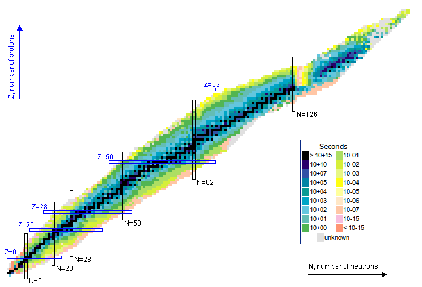
\includegraphics[scale=0.7]{images/stability.png}
\end{center}
 \caption{Stability of the nuclides as a function of the number of protons $Z$and the number of neutrons $N$. Figure taken from \cite{nndc}.}\label{fig:stability}
\end{figure}




\subsection{Decay constants}
If a substance is made of atoms which have a probability $\lambda$ of decaying per time unit, the change of the number of atoms is given by
\[\frac{dN}{dt}=-\lambda N\;,\qquad\Rightarrow \quad N=N_0 e^{-\lambda t}\]
$\lambda$ is called the decay constant. If we want to obtain the mean life we consider the number of decays in a small time interval $dt$: $dN=\lambda N(t)\,dt$ these decays happen at time $t$ so in order to get the mean of the time before decay we need to weight this number of decays by the time $t$, to take all atoms into account we integrate over $t$ and normalise by the total number of atoms:
\[\tau\equiv<t>=\frac{1}{N_0}\int\limits_{0}^{N_0} t dN =\frac{1}{N_0}\int\limits_0^\infty t \lambda N_0 e^{-\lambda t}\,dt=-\lambda\int\limits_0^\infty\frac{1}{-\lambda}e^{-\lambda t}=\frac{1}{\lambda}\]
the mean time before decay is called the lifetime. Another time describing the decay is the so-called half time. It is defined as the time after which half of the elements of the sample will have decayed. It is different from the lifetime but is related through
\[e^{-\lambda t_{1/2}}=\frac12 \quad\Rightarrow \quad t_{1/2}=\frac{\ln(2)}{\lambda}=\tau \ln(2)\]
Figure \ref{fig:decayConstant} shows the exponential decay of the number of nuclei and the lifetime and half time.
%%\image{decayConstant.png}
\begin{figure}
\begin{center}
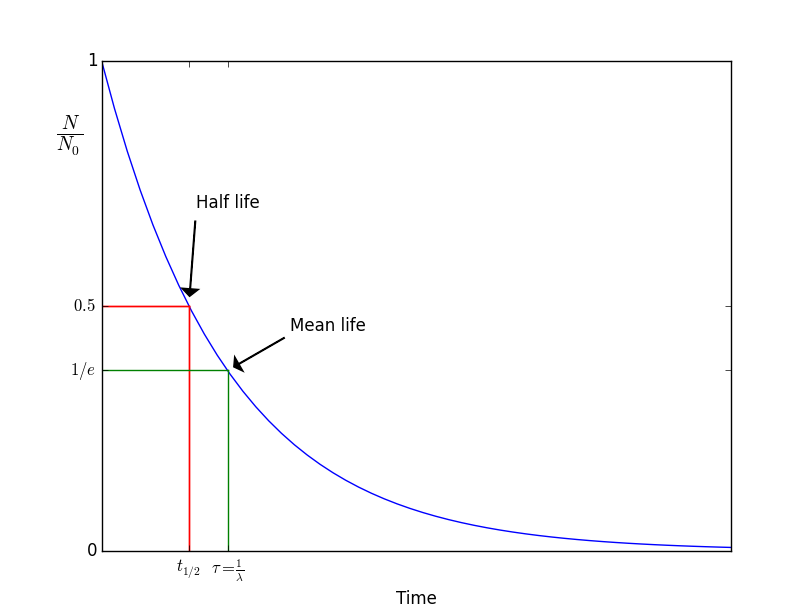
\includegraphics[scale=0.5]{images/decayConstant.png}
\caption{Fraction of atoms remaining as a function of time.}\label{fig:decayConstant}
\end{center}
\end{figure}
The frequency of decays in a material is called the \emph{activity}
\[A=-\frac{dN}{dt}=\lambda N\]
Commonly used units for the activity are Becquerel ($1 Bq=1\;\mbox{decay}/s$) or Curie ($1 Ci=3.7\cdot 10^{10}\;\rm Bq$). The activity of a sample decreases with time as the number of candidate nuclei for a decay diminishes.
\[A(t)=\lambda N(t)=\lambda N_0 e^{-\lambda t}\;.\]
To measure the lifetime of a substance one can either measure the time dependence of the activity or use the definition, the former only practical for relatively short-lived nuclei and the latter requiring a good knowledge of the number of nuclei of a given substance in the sample.
%
%
%
%%\lecture{3}
\subsection{$\beta$-decay}
%
%
%
As a free particle the neutron has a lifetime of about $881.5\,\rm{s}$ and decays into a proton, an electron and a neutrino through the weak force. 
\begin{equation}\label{eq:beta}
n\rightarrow p+e^-+\bar{\nu}_e
\end{equation}
this process is called a $\beta$ decay and it explains why there is no free neutrons while there are free protons (in hydrogen atoms). Neutron can be long lived when they are part of a bound state in a nucleus. Neutrons in the nucleus can still decay into protons if it is energetically favoured. In fact the opposite effect can also happen if the nucleus resulting from a proton changing into a neutron is less massive. This can be the case since loosing a proton reduces the Coulomb energy and depending on the neutron-proton imbalance may result in the newly created neutron taking a lower energy state than the proton. Nuclei with large number of protons will tend to exchange protons for neutrons and nuclei with large numbers of neutrons compared to protons will tend to exchange protons for neutrons. This processes called $\beta$-decay do not change the mass number $A$ but changes $Z$. 

Three processes are possible, all using variations of the $\beta$-decay formula (\ref{eq:beta}) by moving particles between final and initial state. All of them include neutrinos whose mass can be neglected. We will talk about neutrinos in greater details later.
\begin{description}
\item[$\beta^-$ decay:] A neutron in the nucleus decays into a proton, an  electron and an electron anti-neutrino. 
\[n\rightarrow p+e^-+\bar{\nu}_e\]
Such a decay is possible if the mass difference between the parent and daughter nuclei is large enough to "afford" the creation of the electron an neutrino. In terms of atom masses the condition is :
\[M(Z,A) > M(Z+1,A)\]
where the fact that we use atom masses takes the additional electron produced in the decay into account since the daughter nucleus has one more electron than the parent. 
\item[$\beta^+$ decay:] A proton in the nucleus is changed into a neutron by emitting a positron and a neutrino:
\[p\rightarrow n+e^++\nu_e\]
For this process to happen the mass difference between the nuclei should be large enough to "buy" the mass of the positron. In terms of atomic masses the condition is 
\[M(Z,A) > M(Z-1,A) + 2m_e\] 
we need to add twice the mass of the electron on the right-hand side, once to get the mass of the positron, and once to make up for the fact that the nucleus on the left-hand side has $Z$ electrons and the one on the right-hand side has $Z-1$ electrons. 
\item[electron capture:] in this case we consider the case in which an electron from the atom combines with a proton to give a neutron and a neutrino:
\[p+e^-\rightarrow n+\nu_e\]
for this process to occur the condition is less stringent because no energy is needed to produce a positron or electron, only the (negligible) energy for the neutrino is needed. The condition is 
\[M(Z,A)> M(Z-1,A)+\epsilon\]
where $\epsilon$ is the energy of the excited state of the nuclide $\ce{^{A}_{Z-1}X}$ produced. For this process to happen there needs to be some overlap between the electron wave function and the nucleus. This is more likely to be the case for $s$-shell electron since there the radial wave function has a non-zero value at the origin. Also the higher the charge of the nucleus the closer the electron wave function is concentrated close to the nucleus, so electron capture gets more likely for larger nuclei. Electron capture is always possible when $\beta^+$-decay is allowed but the reverse is not true: if the mass difference between two isobars is smaller than $2m_e$ only electron capture is possible.
\end{description}

Since these decays do not change $A$ we can quantify this by looking at the semi-empirical formula eq.~\ref{eq:SEMF} for a fixed value of $A$. Substituting $N=A-Z$ we find that the mass formula is quadratic in $Z$ so we expect the masses of the isobars to fit on a parabola. 
\begin{figure}
\begin{center}
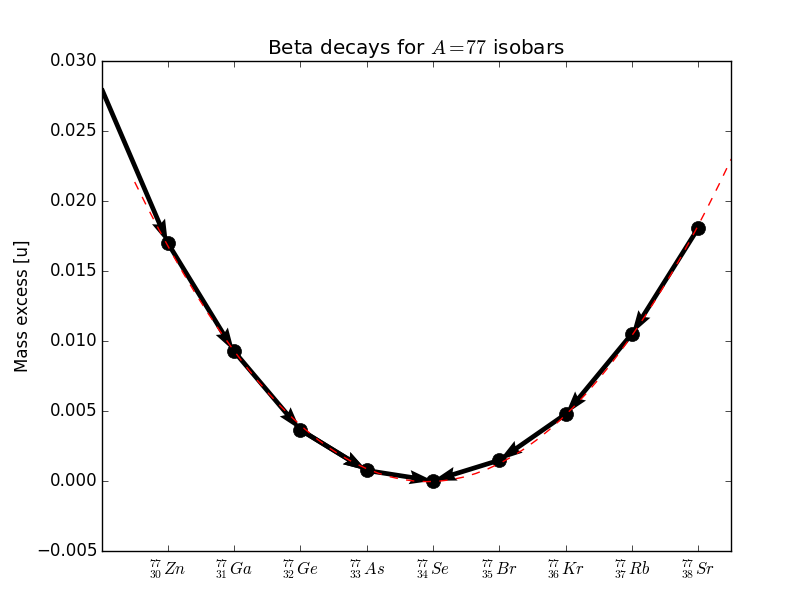
\includegraphics[scale=0.4]{images/isobar77.png}
%%\image{isobar80.png}
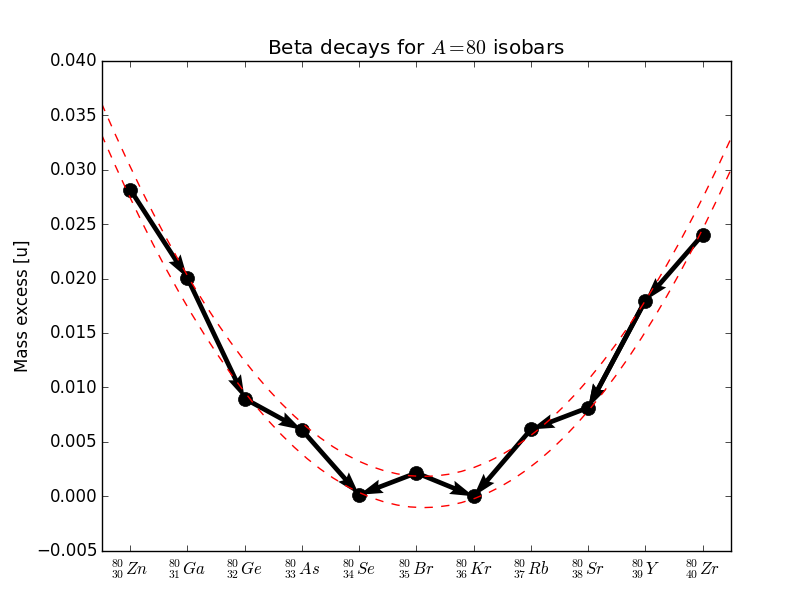
\includegraphics[scale=0.4]{images/isobar80.png}
\end{center}
\caption{Mass differences between isobars and the lightest isobar for $A=77$ (left) and $A=80$ (right). The arrows represent $\beta$-decays.}\label{fig:isobars}
\end{figure}
In the case of odd $A$ we have one parabola, as shown in Figure~\ref{fig:isobars}. In such a case only one isobar is the lowest and is $\beta$-stable. All other isobars can decay to that stable isobar. 

In the case of even $A$ nuclei there are two parabolas because of the pairing term. An example is shown in Figure~\ref{fig:isobars}. In some cases we are in a situation where there are two nuclides of the even-even type lower than a nuclide of odd-odd type. 
%%\keypoint{Nuclei can exchange a neutron for a proton in a $\beta^-$ decay.}
%%\keypoint{Nuclei can exchange a proton for a neutron in a $\beta^+$ decay.}
%%\keypoint{Nuclei can capture an electron in the atom to change a proton in a neutron.}
%
%
%
\subsection{$\alpha$-decay}
%
%
%
Another possibility for decay is the $\alpha$-decay where an $\ce{^4He}$ nucleus, also called $\alpha$-particle is emitted. This decay reduces $Z$ by two units and $A$ by four. For this decay to happen the mass of the atom must satisfy (neglecting the electron mass):
\[M(Z,A)> M(Z-2,A-4)+M(2,4)\]

To investigate the alpha decay we consider an $alpha$-particle within a nucleus for which alpha decay is allowed. The potential the particle is experiencing is sketched on the left-hand side of Figure~\ref{fig:fissionPotentials}. Outside of the nucleus (that is further than the range of the nuclear force) the alpha particle only feels the Coulomb potential of the daughter nucleus. Inside the nucleus the Coulomb potential is stronger and forms the potential well with boundary at distance $r\simeq R$. $\alpha$-decay proceeds through tunnelling through the Coulomb potential barrier. Since the $\alpha$-decay occurs through tunnelling the dependence of the decay time on the energy is exponential, which explains why the lifetimes for $\alpha$-decay cover a very wide range of timescales.    
\begin{figure}
\begin{center}
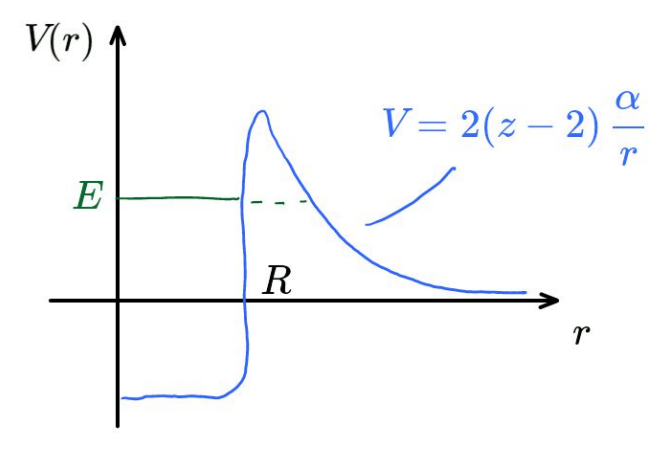
\includegraphics[scale=0.3]{images/alphaDecayPotential.png}
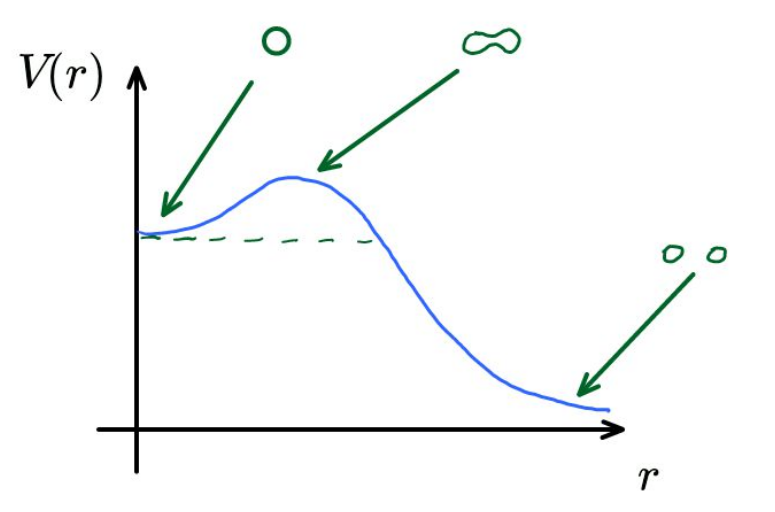
\includegraphics[scale=0.25]{images/fissionPotential.png}
\end{center}
\caption{Left panel: Potential of an $\alpha$-particle as a function of the distance to the nucleus. This is the case where the decay is possible, if it was not possible the energy $E$ would be below $0$. Right panel: Potential for the two daughters in a fission process as a function of the separation.}\label{fig:fissionPotentials}
\end{figure}
%%\keypoint{The $^4He$ nucleus is very stable and can be emitted by an unstable nucleus. Such a decay is called $\alpha$ decay.}
%
%
%%\lecture{4}
\subsection{Nuclear fission}
%
%
%
$\alpha$-decay is only one case in which the nucleus splits into several smaller nuclei. If we look at the energy as we pull the two parts of a nucleus apart we can sketch the potential for the distance of the two part as a function of the distance. Starting from the ground state of the parent nucleus (which we assume to be spherically symmetric) we start stretching the nucleus, this increases the surface energy, because at fixed inner volume, the sphere is the surface with the smallest surface to volume ratio. The Coulomb potential energy on the other hand decreases, eventually dominating the surface energy and the two parts separate. The potential is shown on the right-hand side of Figure~\ref{fig:fissionPotentials}
%%\keypoint{Heavy nuclei can decay spontaneously into smaller parts.}
\begin{figure}
\begin{center}
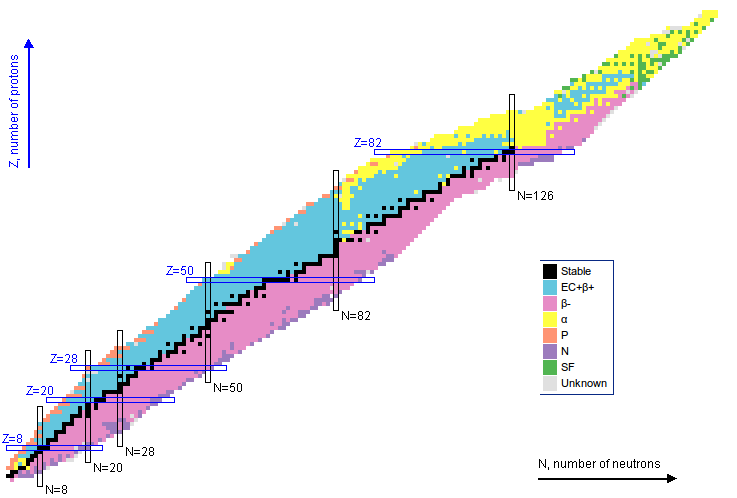
\includegraphics[scale=0.35]{images/decayModesWithLegend.png}   
\end{center}
\caption{Decay modes in the $N$-$Z$ plane. Data from \cite{nndc}}\label{fig:decayModes}
\end{figure} 

The height of the barrier is called the activation energy. Very few nuclides decay through spontaneous fission, in most cases $alpha$-decay is more likely (see Figure~\ref{fig:decayModes}). The probability of fission increases with $Z$ and is more likely for heavy nuclides. Fission processes can be induced by exposing the nuclides to a flux of neutrons. If an atom absorbs a neutron it will acquire its kinetic energy (although part of it will be needed to produce the daughter nucleus recoil) and it also gains the bounding energy associated with the additional neutron. This additional energy can bring the nucleus energy above the fission barrier, triggering the fission of the nucleus. 

Fission is not the only way a nucleus excited through neutron absorption can decay in a stable state. It can also do so through the emission of a photon. This process is called radiative capture. Figure~\ref{fig:neutronCrossSection} shows the cross section for the absorption of a neutron by two isotopes of uranium. Neutrons with energies below the region with the resonances are called called "slow", neutrons with energies above the resonance region are called "fast". For $\ce{^{235}U}$ the fission cross section is larger than that for radiative capture which means that a neutron is most likely to trigger a fission. For $\ce{^{238}U}$ the situation is different, for energies below about $1\;\rm{MeV}$ absorption is most likely happening radiatively, while fission only occurs for energies higher that about $1\;\rm{MeV}$.

%%\image{neutronCrossSection.png}
\begin{figure}
\begin{center}
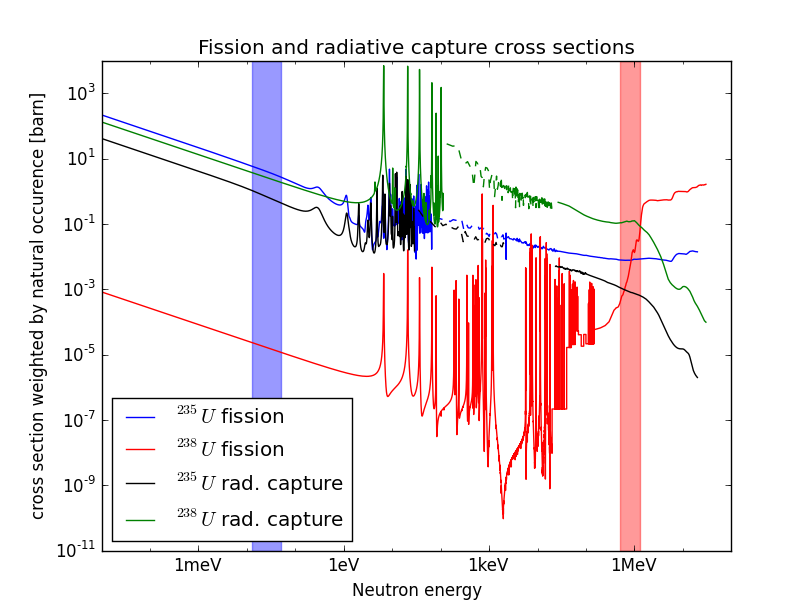
\includegraphics[scale=0.5]{images/neutronCrossSection.png}   
\end{center}
\caption{Cross sections for induced fission and radiative capture for the two main isotopes or uranium. The shaded regions represent the typical energies for thermal neutrons (around 0.025 MeV) and neutrons from the fission process (around 1 MeV). Data from \cite{nds}}\label{fig:neutronCrossSection}
\end{figure} 
Fission of a heavy nucleus usually result in neutron-rich daughter nuclei, some free neutrons and kinetic energy. In the fission of $\ce{^{235}U}$ these neutrons have energies with a peak slightly lower than $1\;\rm{MeV}$. In pure $\ce{^{235}U}$ these neutron can be absorbed by another uranium nucleus that will most likely trigger a new fission. Since the number of neutrons released is larger than one this can generate a chain reaction where the number of neutrons available to trigger a new fission increases exponentially until the residual thermal caused by the kinetic energy of the daughter nuclei cannot be contained. This is the principle of an atomic bomb. 

The fuel used in a nuclear reactor is not pure $\ce{^{235}U}$ but is a mixture of the two uranium isotopes, closer to their natural occurrences ($\ce{^{238}U}$: 99\%,$\ce{^{235}U}$: 0.7\%). If nothing is done to prevent it, secondary neutrons from the fission of an $\ce{^{235}U}$ atom will be in most cases absorbed through radiative capture by $\ce{^{238}U}$ and no chain reaction can be sustained. The idea in a nuclear reactor is to "cool" the neutrons from the fission to energies below the resonance region (where the fission of $\ce{^{235}U}$ is dominant) so that they are available to trigger new fissions. The way neutrons can be cooled is to let them propagate through a medium that will not absorb them, but will reduce their kinetic through elastic scatterings. Such a medium is called a moderator. The ideal properties of a moderator is that it should not absorb neutrons easily and it should be efficient at reducing the kinetic energy of the neutrons. The first property is fulfilled by materials rich in neutron. For the second property we want that the free neutron loses as much energy as possible at each elastic scattering. This is best obtained for light nuclei (in the case of an extremely heavy nuclei the neutron energy would not change at all). Graphite (carbon) and heavy water ($D_2O$) are good moderators used in practice. The arrangement depicted in Figure~\ref{fig:reactor} that allows for a sustained reaction is to have fissible fuel separated in a volume of moderator.       
\begin{figure}
\begin{center}
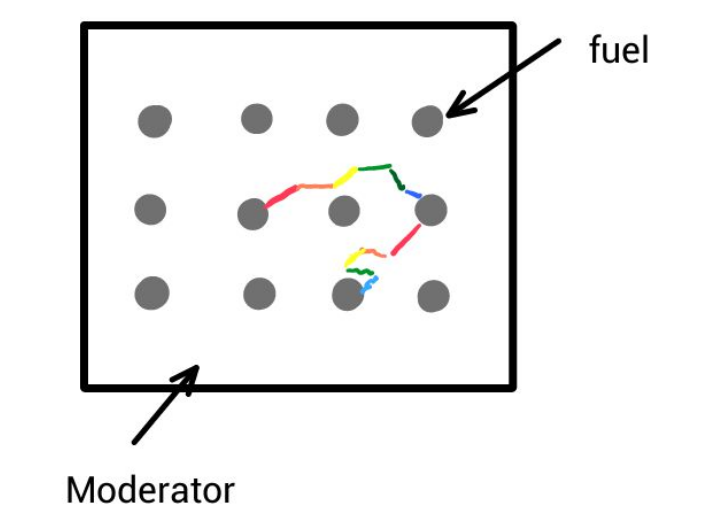
\includegraphics[scale=0.3]{images/reactor.png}   
\end{center}
\caption{Moderator and fuel arrangement in a nuclear reactor.}\label{fig:reactor}
\end{figure} 
\clearpage
%%\keypoint{A suitable arrangement of fissible material and moderator can sustain a controlled chain reaction.}
%
%%\lecture{5}
%%\section{The Shell Model}
\subsection{Shell model}
%
%
%
So far we have investigated the mass and stability of nuclei, now we want to explore the structure of the nucleus in more details. We understand the effects of the mass number $A$ and the number of protons and neutrons $Z$ and $N$ on the strength of the binding of the nuclei but when we look at the energy it takes to excite nuclei to their first excited state we see that the largest excitation energies are concentrated around specific values of $N$ and $Z$, see Figure~\ref{fig:firstExcited}.  
\begin{figure}
\begin{center}
%%\image{firstExcitedStateEnergyWithLegend.png}
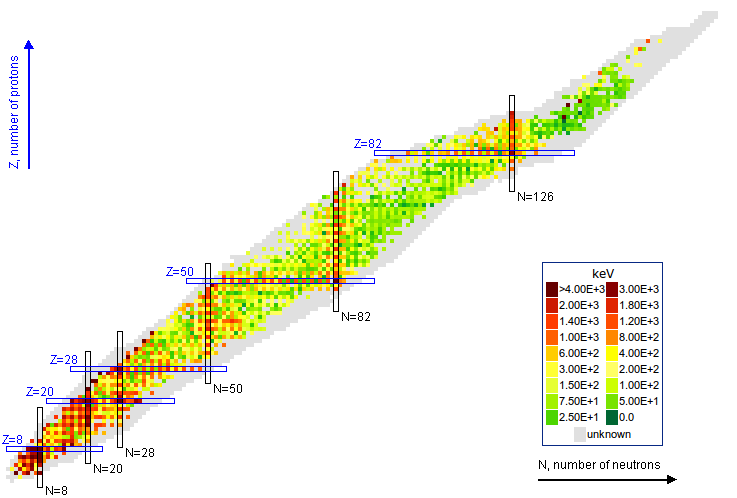
\includegraphics[scale=0.4]{images/firstExcitedStateEnergyWithLegend.png}
\end{center}
\caption{First excited state energy. The highest energies (and hence the most stable states) are concentrated around proton and neutron numbers equal to 2,8,20,28,50,82,126}\label{fig:firstExcited}
\end{figure}
These numbers are called "magic" numbers. The shell model can explain these numbers. We already observed that the binding energy per nucleon had enhancements around the places corresponding to one of the proton or neutron number close to a magic number.

For the shell model we consider a nucleon moving in the potential generated by the other nucleons. The potential will have discrete energy levels and since the nucleons are fermions there will be at most two nucleons in the same state. Since protons and neutrons are different fermion this limitation is only acting on the protons and neutrons as separate groups so we will get separate spectra for each type of nucleon. We assume that the nuclear potential is spherically symmetric so the wave functions can be expressed in terms of spherical harmonics. The solutions can be labelled by two quantum numbers, one enumerating the solutions of the radial wave-function, $n=1,2,3,...$ and the angular momentum $l=0,1,2,3,...$. We will use the spectroscopic nomenclature $l=s,p,d,f,...$ to label the orbital momentum quantum number. 

If the potential can be approximated by an harmonic oscillator the energy would be given by the usual
\[E=\left(2n+l-\frac{1}{2}\right)\omega\] 
If we approximate it as an infinite well potential we obtain the levels depicted in Figure~\ref{fig:levels}.

\begin{figure}
\begin{center}
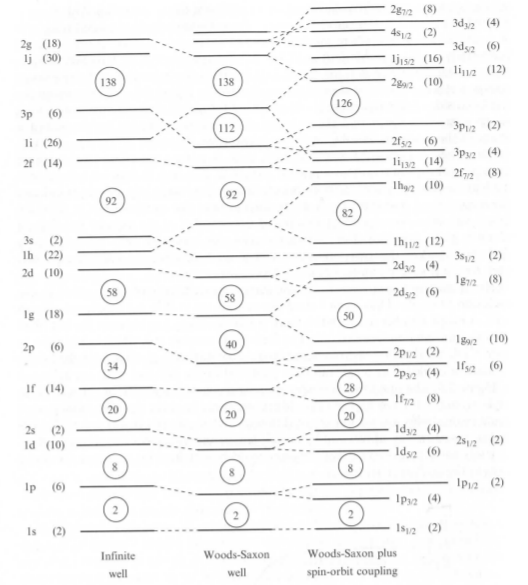
\includegraphics[scale=0.5]{images/harmonicSWplusSpinCoupling.png}
\caption{Energy levels in an infinite potential well, in the Saxon-Woods potential before and after including the spin-orbit coupling. Figure taken form \cite{Lilley:2009zz}, p.48.}\label{fig:levels}
\end{center}
\end{figure}

Unfortunately the actual nuclear potential is neither harmonic nor an infinite well. Since the nuclear force is very short range, the potential it creates should follow the density of nucleons in the nucleus. We will see later which form this density takes and how to measure it. Empirically we can use the following form 
\[V(r)=-\frac{V_0}{1+e^{(r-r_0)/a}}\]
with parameters $r_0$ and $a$ fitted from data. With this potential we obtain the levels shown in the central part of Figure~\ref{fig:levels}. This potential alone is not enough to describe the features that the mass spectrum of nuclides displays. Although the first magic numbers are predicted properly the gap between energy levels do not line up properly to explain the higher magic numbers.

To achieve the agreement with the data we need to consider an addition to the potential: the spin-orbit coupling. In the hydrogen atom electron energy levels the interaction caused by the spin-orbit term in the potential is responsible for the hydrogen fine structure. In the hydrogen case it is not a large effect. In the case of the shell model of the nucleus the effect is larger and does not only creates a splitting but actually reorders shells of different $n.l$ quantum numbers, which places the gabs in the energy levels at the right place to explain the magic numbers. The spin-orbit coupling term is given by 
\[V_{SO}=V_{ls}(r)\left<\vec{l}\cdot\vec{s}\right>\] 
We can calculate the expectation value of the expectation value of $\vec{l}\cdot\vec{s}$ as a function of the eigenvalues of the total angular momentum $j$:
\[
j(j+1)=\left<\vec{j}^2\right>=\left<(\vec{l}+\vec{s})^2\right>
=
\left<\vec{l}^2+2\vec{l}\cdot\vec{s}+\vec{s}^2\right>
=l(l+1)+s(s+1)+2\left<\vec{l}\cdot\vec{s}\right>
\]
\[\Rightarrow
\left<\vec{l}\cdot\vec{s}\right>=\frac{j(j+1)-l(l+1)-s(s+1)}{2}
\]
according to the rules of angular momentum addition the possible values of $j$ are either $l+1/2$ of $l-1/2$ so we get
\[\left<\vec{l}\cdot\vec{s}\right>=\left\{\begin{array}{rcc}
l/2&\mbox{for}& j=l+1/2\\
-(l+1)/2&\mbox{for}& j=l-1/2
\end{array}\right.\]
As for the hydrogen atom, we can now label the levels with $n,l$ and $j$. The quantum number $l$ determines the parity of the state. The energy split between the two $j$ levels is given by
\[
\Delta E_{SO,ls}=\left<V_{ls}(r) \vec{l}\cdot\vec{s}\right>=
\left(\frac{l}{2}-\frac{-(l+1)}{2}\right)=\left<V_{ls}(r)\right>\frac{2l+1}{2}
\]
We find experimentally that the coefficient $\left<V_{ls}(r)\right>$ is negative so that unlike for the electron levels in the hydrogen the energy level with the higher value of $j$ is the lower lying one. The result of including this contribution is shown on the right of Figure~\ref{fig:levels} and result in splits between levels consistent with the magic numbers. 
%%\keypoint{The spin-orbit interaction in the nucleus is much stronger than in the hydrogen atom and has opposite sign.}
In practice the proton and neutron potentials can have slightly different shapes resulting in small differences in the ordering of the shells within a band, but not affecting the magic numbers, see Figure~\ref{fig:pnlevels}. 

%%\image{Shell.png}   
\begin{figure}
\begin{center}
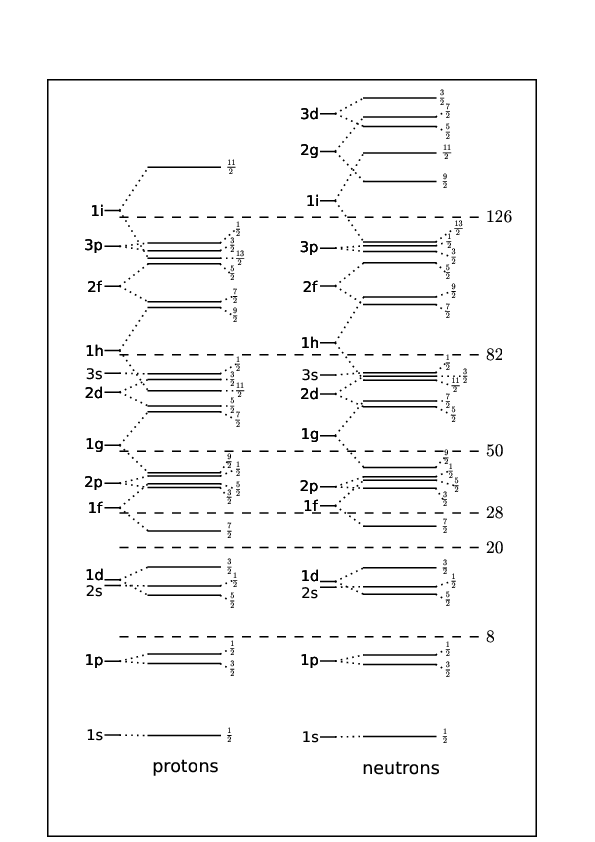
\includegraphics[scale=0.5]{images/Shell.png}
\caption{Energy levels for protons and neutrons. The ordering within a band are different for higher levels, but the structure in bands with magic number of nucleons is the same.}\label{fig:pnlevels}
\end{center}
\end{figure}

The shell model is successful at explaining the magic numbers, but it can also predict (albeit with less success) the spin and parity of the nuclei. 
%%\keypoint{The shell model can explain the magic numbers and predict spin and parity of ground state of nuclei, as well as some excited states.}
%%\lecture{6}
\subsection{Spin and parity of nuclei}

Assuming that the potential is spherically symmetric we could express the angular part of the wave functions to be spherical harmonics $Y_{l,m}(\theta,\phi)$. These functions behaves as
\[Y_{l,m}(\theta,\phi)\rightarrow (-1)^l Y_{l,m}(\theta,\phi)\]
under the parity transformation $\mathbf{P}$ that takes $\vec{r}$ to $-\vec{r}$. Experimental evidence supports the fact that the strong and electromagnetic forces conserve parity so we can expect parity to be a conserved quantum number for the nucleus states. With our labelling with $l$ the parity of a state can be directly read off as $(-1)^l$.

If a shell is full we expect all contributions to the angular momentum to cancel out and the parity to be $+1$ as there is an even number of particles in the full shell. Let's now look at what happens if we have a full shells up to one additional nucleon. We can apply our "one particle in the potential of the other" analysis of the shell model and predict that the spin and parity of the nucleus will be determined by the parity and angular momentum of this nucleon, so the spin will be $0,1,2,3,...$ if the single nucleon is in a $s,p,d,f,...$ state. Its parity will be $(-1)^l$, that is $+1$ for $s,d,g,..$ shells and $(-1)$ for $p,f,h,...$ shells. 

If we have full shells up to one missing nucleon, then the spin and parity will be determined by the angular momentum and parity of the missing nucleon (often referred to as "hole").

Using the fact that nucleons tend to pair we can extend this analysis to shells that are further to being full than by one nucleon. We can assume that the contributions from paired nucleons will cancel and only the unpaired nucleon contributes to the spin and parity of the nucleus. 

The shell model gives predictions for even-even nuclei: they will all have $J^P=0^+$, for odd-even nuclei the spin and parity is given by the odd nucleon. The situation is more complicated for odd-odd nuclei where no clear prediction can be made from the shell model.  
%%\image{levels_17F.png}
\begin{figure}
\begin{center}
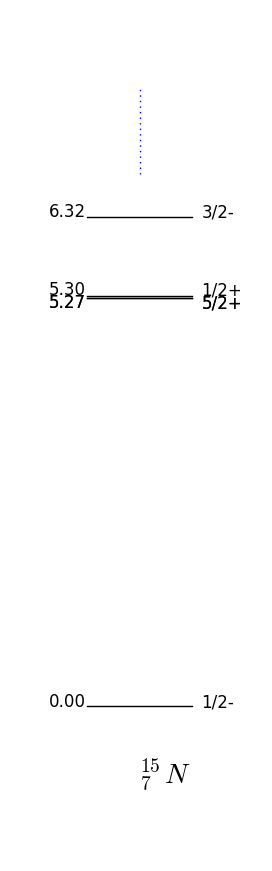
\includegraphics[scale=0.4]{images/levels_15N.png}
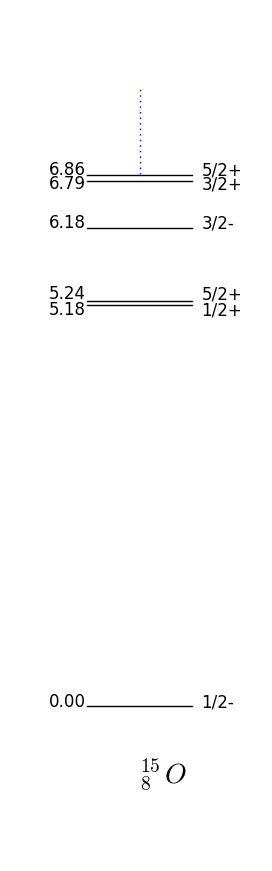
\includegraphics[scale=0.4]{images/levels_15O.png}
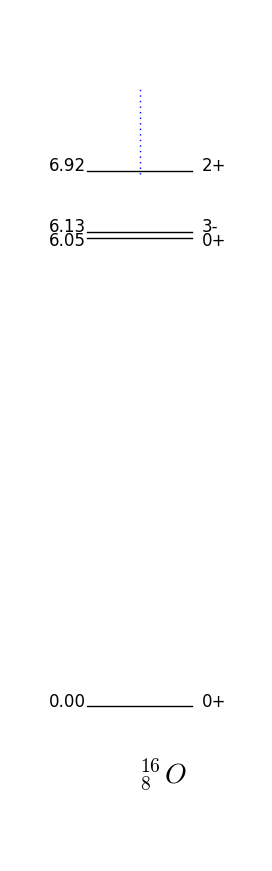
\includegraphics[scale=0.4]{images/levels_16O.png}
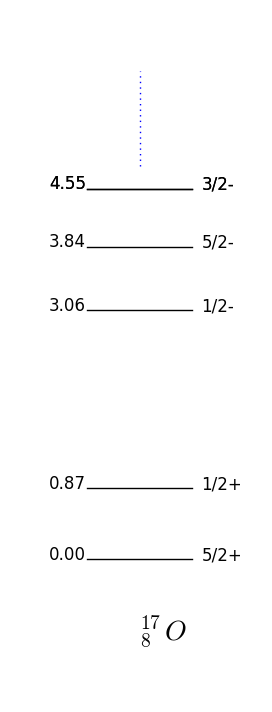
\includegraphics[scale=0.4]{images/levels_17O.png}
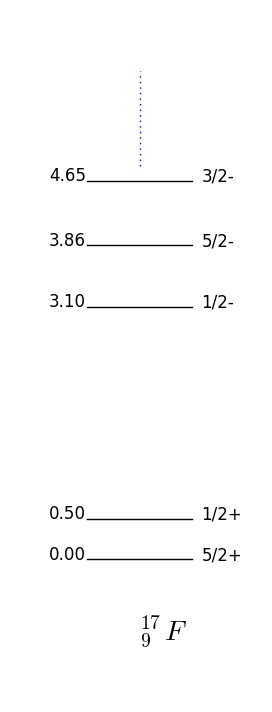
\includegraphics[scale=0.4]{images/levels_17F.png}
\caption{Energy levels for nuclei with proton and neutron numbers close to the magical number 8.}\label{fig:levelsNOOOF}
\end{center}
\end{figure}

With the shell model we can also explain some of the spin and parity of excited levels of nuclei. Figure~\ref{fig:levelsNOOOF} shows the energies and $J^P$ quantum numbers of excitations of nuclei with proton and neutron numbers close to the magical number $8$. Let us look at these nuclei in turn. $\ce{^{16}O}$ has full shells for both neutrons and nucleons. It is therefore very stable and its ground state has $J^P=0^+$.

$\ce{^{15}N}$ has 8 neutrons so the neutron $1s$ and $1p$ shells are full. It has 7 protons so we have a full $1s$ shell, a full $1p_{3/2}$ shell but a hole in the $1p_{1/2}$ shell. We therefore expect the spin and parity of the ground state to be $J=1/2$ and $P=(-1)^1=-1$.\footnote{One could have argued the other way and say the unpaired proton is in the $1p_{1/2}$ shell, instead of looking for the shell of the hole.}

$\ce{^{15}O}$ and $\ce{^{17}N}$ are called \emph{mirror nuclei} because they map into each other through swapping the protons with neutrons.
%
%
%
\subsection{Excited states}
%
%
%
Nuclei have many excited states. We have seen that some of them can be explained by the shell model. There are also other excited states that correspond to vibrational or rotational excitations. 

%%\keypoint{Nuclei in excited states can relax to lower lying states through the emission of photons. This process is called $\gamma$-radiation.} 
An excited nucleus can relax into its ground state through emission of a photon. Conversely a photon can be absorbed to move such a system from one energy state to a higher one. In this section we will consider the case of a decay, the discussion of the other case is similar. The relevant ingredient for this process are the parity, spin, orbital and total angular momentum of the initial and final states. The emitted photon can (actually it has to) carry away some angular momentum, we denote this amount with $\ell$. It is related to the multipolarity of the radiation: $\ell=1$ is called dipole radiation, $\ell=2$ quadrupole, $\ell=3$ octopole, etc. Angular momentum has to be conserved, so we have
\[\vec J_p=\vec J_d+\vec \ell\]
with $\vec J_p$ and $\vec J_d$ the total angular momentum of the parent and daughter states. Because of this constraint we have
\[|J_p-J_d|\leq \ell \leq J_p+J_d \;.\]
It is important to note that this equation leads to results that can appear counter-intuitive. For example for $J_p=J_d=1$ we can have $\ell=2$. It would appear that the angular momentum did not change and yet the photon carries some angular momentum away. The important point is that this is a vector equation and in this case $\vec J_p=-\vec J_d$ and while they have the same norm their angular momentum did change as a vector. In other words one can have $\Delta J=0$ with $\Delta \vec J\neq 0$. 

There are two ways for the initial state to change its angular momentum, it can change its spin or change its orbital angular momentum. If a spin change has occurred, the transition is classed as ``magnetic'' if not it is called ``electric''. A transition with change on angular momentum $\ell=|\vec{\ell}|$ is labelled $E\ell$ or $M\ell$ if it is electric or magnetic. It turns out that the matrix element for a change of spin is typically smaller than that of changing the orbital momentum, so magnetic transitions are normally less likely than the electric transitions for the same $\ell$. The higher $\ell$ is the least likely the transition is so that transitions will normally take part with the lowest $\ell$ allowed by the conservation constraints.

Let us now consider the effect of parity. To calculate the parity of the final state we have to combine the parity of the daughter state $P_d$ and the parity of the EM radiation. The parity of the EM radiation depends on whether its origin is electric or magnetic. It is $(-1)^\ell$ for an electric transition and $(-1)^{\ell+1}$ for magnetic transitions. So we have for the parity $P_p$ of the parent state:
\[P_p=\left\{\begin{array}{cc}
P_d(-1)^\ell&\mbox{for $E$ transitions}\\
P_d(-1)^{\ell+1}&\mbox{for $M$ transitions}
\end{array}\right.
\]

The above facts give us the following selection rules for $\ell=1$ transitions:
\[|J_i-J_f|\leq 1\leq J_f+J_i \qquad\mbox{and}\qquad P_p=\left\{\begin{array}{cc}
-P_d&\mbox{for an $E1$ transition}\\
+P_d&\mbox{for a $M1$ transition}\end{array}\right.\]
That is the difference between the $J$ values of the daughter and parent states cannot be larger than $1$ (so it can be $0$ or $1$) and their sum has to be larger than $1$. For an electric transition this is accompanied by a change of parity and for a magnetic transition the parity of the daughter particle has to be the same as that of the parent.

Let us now look at $\ell=2$ transitions. The above facts give us the following selection rules:
\[|J_i-J_f|\leq 2\leq J_f+J_i \qquad\mbox{and}\qquad P_p=\left\{\begin{array}{cc}
+P_d&\mbox{for an $E2$ transition}\\
-P_d&\mbox{for a $M2$ transition}\end{array}\right.\]
That is the difference between the $J$ values of the daughter and parent states cannot be larger than $2$ ($0$, $1$ and $2$ are possible), and their sum has to be larger than $2$. For a magnetic transition this is accompanied by a change of parity and for an electric transition the parity of the daughter particle has to be the same as that of the parent. 

Given a parent and a daughter states, one can find the transitions by first listing all allowed $\ell$ according to
\[|J_i-J_f|\leq \ell\leq J_f+J_i\;; \]
for each $\ell$ only one of the $E$ and $M$ transitions will be allowed by parity. If a $E\ell$ transition is allowed, parity will allow transitions $E(\ell\pm2),E(\ell\pm4)...$ and $M(\ell\pm1),M(\ell\pm3)...$, but angular momentum conservation will not allow all of them. We will often find situations where $E\ell$ and $M(\ell\pm1)$ are allowed and wonder which one is most likely. The case $E\ell/M(\ell+1)$ is easy as $E$ transitions are more likely than $M$ transitions and the likelihood is decreasing strongly with increasing $\ell$. The other case with $M\ell$ and $E(\ell+1)$ is more complicated and the two can be of similar size, leading to interference effects.  
\pagebreak
\section{Key Points}
\begin{itemize}
\item The masses of the nuclei can be approximately described by the semi-empirical mass formula (SEMF).
\item The nuclear force is short range and creates a more or less constant potential within the nucleus volume
\item Nucleons at the boundary of the nucleus volume have fewer neighbours and therefore their binding energy is smaller.
\item Protons in the nucleus experience a repulsive Coulomb force due to their positive charges.
\item Protons and nucleons prefer to be in pairs in the nucleons, it gives rise to the pairing term.
\item Nuclei can exchange a neutron for a proton in a $\beta^-$ decay. 
\item Nuclei can exchange a proton for a neutron in a $\beta^+$ decay. 
\item Nuclei can capture an electron in the atom to change a proton in a neutron. 
\item The $\ce{^4He}$ nucleus is very stable and can be emitted by an unstable nucleus. Such a decay is called $\alpha$ decay.
\item The shell model can explain the magic numbers and predict spin and parity of ground state of nuclei, as well as some excited states.
\item The spin-orbit interaction in the nucleus is much stronger than in the hydrogen atom. 
\item Nuclei in excited states can relax to lower lying states through the emission of photons.
\end{itemize}
\subsection{Quick question}
\begin{itemize}
\item What is the source of the asymmetry term in the SEMF?
\item Which process has kinematic constraints easiest to satisfy? $\beta^+$ or electron capture decay?
\item Why does one need a moderator in a nuclear reactor?
\item What is the spin and parity of $\ce{^{18}_{8}O}$?
\item What is the maximum and minimum multipolarity of a transition between $J_1=2$ and $J_2=5$ states? 
\end{itemize}
\pagebreak
\appendix
%%\section{Advanced topics}
\section{A possible derivation of the Coulomb term}
We can derive an approximate formula for the Coulomb term in the semi-empirical mass formula as follows. If we split the $Z$ units of charge into infinitely many parts of charge $dz$ and consider the energy needed to bring them from an infinite distance to the place where we reconstitute the nucleus with a fixed density of charge $\rho$ we find that the energy is given by 
\[dE\frac{e^2 z\,dz}{4\pi\epsilon_0 r(z)}\]
where $z$ is the amount of charge already present. Since we have a constant density, the radius as a function of $z$ is given by
\[\rho=\frac{3 z}{4\pi r(z)^3}\qquad \Rightarrow \qquad r(z)=\left(\frac{3z}{4\pi\rho}\right)^{\frac{1}{3}}\]
To obtain the total energy we need to integrate $z$ from 0 to the total charge:
\[E=\frac{e^2}{4\pi\epsilon_0}\int\limits_0^{Z}\left(\frac{4\pi\rho}{3}\right)^{\frac{1}{3}}z^{2/3}\,dz=\frac{e^2}{4\pi\epsilon_0} \left(\frac{4\pi\rho}{3}\right)^{\frac{1}{3}}\frac{3}{5}Z^{5/3}\] 
The density $\rho$ is given by:
\[\rho=\frac{3Z}{4\pi R^3}\,,\]
where $R$ is the radius of the nucleus. Plugging this in we get:
\[E=\frac{3\alpha Z^2}{5 R}\] 
which has the almost the right $Z$ dependence. The difference with the term in the semi-empirical formula eq.~\ref{eq:SEMF} is that in this calculation we have accounted for the energy to "assemble" a proton, but this energy is already present in the mass of the proton so we are slightly overestimating the Coulomb energy.   




\bibliographystyle{IEEE}
\bibliography{bibliography}

\end{document}
